% \iffalse meta-comment
%
% Copyright (C) 2021-2022 MeteoSwiss, originally written by Frédéric P.A. Vogt
%
% This file may be distributed and/or modified under the
% conditions of the BSD-3-Clause License.
% The terms of this license are available at:
%
% https://opensource.org/licenses/BSD-3-Clause
%
% SPDX-License-Identifier: BSD-3-Clause
%
%
% \fi
%
% \iffalse
%<package>\NeedsTeXFormat{LaTeX2e}[2005/12/01]
%<package>\ProvidesPackage{metsymb}
%<package>     [2022/09/10 v1.2 The meteorological symbols package]
%
%<*driver>
\documentclass{ltxdoc}
\usepackage[margin=1.2in]{geometry} % For more reasonable margins
\usepackage{tocloft} % For a better table of content in the doc
\renewcommand{\cftsecleader}{\cftdotfill{\cftdotsep}} % Idem
\usepackage{color} % For using colors
\usepackage{tabularx} % For the tables
\usepackage{graphicx} % For the demo Python plot
\usepackage{listings}% For including code
\lstset{
  basicstyle=\footnotesize,        % the size of the fonts that are used for the code
  frame=single,                          % add a frame around code
  }
\usepackage{hyperref} % For the colored table of contents
\hypersetup{
    colorlinks=true,
    linkcolor=red,
    %filecolor=magenta,
    urlcolor=blue,
    %pdftitle={Overleaf Example},
    %pdfpagemode=FullScreen,
    }
\usepackage{amsmath} % For proper mathematical notations
\usepackage{metsymb}
\EnableCrossrefs
\CodelineIndex
\RecordChanges
\begin{document}
\DocInput{metsymb.dtx}
\end{document}
%</driver>
% \fi
%
% \CheckSum{188}
%
% \CharacterTable
% {Upper-case \A\B\C\D\E\F\G\H\I\J\K\L\M\N\O\P\Q\R\S\T\U\V\W\X\Y\Z
% Lower-case \a\b\c\d\e\f\g\h\i\j\k\l\m\n\o\p\q\r\s\t\u\v\w\x\y\z
% Digits \0\1\2\3\4\5\6\7\8\9
% Exclamation \! Double quote \" Hash (number) \#
% Dollar \$ Percent \% Ampersand \&
% Acute accent \' Left paren \( Right paren \)
% Asterisk \* Plus \+ Comma \,
% Minus \- Point \. Solidus \/
% Colon \: Semicolon \; Less than \<
% Equals \= Greater than \> Question mark \?
% Commercial at \@ Left bracket \[ Backslash \\
% Right bracket \] Circumflex \^ Underscore \_
% Grave accent \` Left brace \{ Vertical bar \|
% Right brace \} Tilde \~}
%
%
% \changes{v1.1}{2022/09/10}{Changelog moved to https://github.com/MeteoSwiss/metsymb}
% \changes{v1.0}{2021/08/26}{Initial version, with okta and cloud symbols.}
%
% \GetFileInfo{metsymb.sty}
%
% \DoNotIndex{}
%
% \title{The \textsf{metsymb} package\thanks{This document
% corresponds to \textsf{metsymb}~\fileversion,
% dated \filedate.}}
% \author{Frédéric P.A. Vogt \\ \texttt{frederic.vogt@meteoswiss.ch}}
%
% \maketitle
%
% \begin{abstract}
% \noindent This package introduces commands to generate professional meteorological symbols with vectorial quality. As of \today, these include: oktas (\zerookta, \oneokta, \twooktas, \ldots), cloud genera (\cirrus, \cirrostratus, \nimbostratus, ...), and C$_\text{L}$--C$_\text{M}$--C$_\text{H}$ cloud codes (\clIII, \cmVI, \chIX, \ldots). This package essentially introduces a new font in which each symbol is assigned to a glyph, which can then be called individually from \LaTeX\ documents via dedicated commands.
% \end{abstract}
%
% \tableofcontents
%
% \section{Introduction}
%
% The creation of this package was motivated by the fact that in 2021, there were no dedicated Unicode elements for \href{https://en.wikipedia.org/wiki/Okta}{okta} and \href{https://cloudatlas.wmo.int/en/abbr-and-symbols-of-clouds-table-genera-species.html}{cloud genera} symbols. To the best of my knowledge, no \LaTeX\ package provides a uniform set of these symbols either\footnote{If you know of one, please let me know and I shall list it here !}.\\
%
% \noindent This package is a direct attempt to remedy to this unfortunate state of affair. Individual symbols are designed using TikZ\footnote{\url{https://www.ctan.org/pkg/pgf}}. They are then bundled into a dedicated font with FontForge\footnote{\url{https://fontforge.org/en-US/}}. Individual glyphs of this metsymb font are then tied to dedicted \LaTeX\ commands via this package.
% \newpage
% \section{Usage}
%
% Using the \textsf{metsymb} package is straightforward. By importing it via a not-so-surprising \texttt{\textbackslash usepackage\{metsymb\}} in the preamble of your documents, you will gain access to the commands listed in Tables~\ref{tbl:oktas} to \ref{tbl:clcmch}.
%
% \begin{table}[htb!]
% \centering
% \caption{\textsf{metsymb} commands for the okta symbols.}\label{tbl:oktas}
% \vspace{5pt}
% \begin{tabular}{c l c l}
% \zerookta & |\zerookta| &  \fiveoktas & |\fiveoktas|\\
% \oneokta & |\oneokta| & \sixoktas & |\sixoktas|\\
% \twooktas & |\twooktas| & \sevenoktas & |\sevenoktas|\\
% \threeoktas & |\threeoktas| & \eightoktas & |\eightoktas|\\
% \fouroktas & |\fouroktas| & \nineoktas & |\nineoktas|
% \end{tabular}
%\end{table}
%
% \begin{table}[htb!]
% \centering
% \caption{\textsf{metsymb} commands for the cloud genera symbols.}\label{tbl:clouds}
% \vspace{5pt}
% \begin{tabular}{c l c l}
% \cirrus & |\cirrus| &  \nimbostratus & |\nimbostratus|\\
% \cirrocumulus & |\cirrocumulus| & \stratocumulus & |\stratocumulus|\\
% \cirrostratus & |\cirrostratus| & \stratus & |\stratus|\\
% \altocumulus & |\altocumulus| & \cumulus & |\cumulus|\\
% \altostratus & |\altostratus| & \cumulonimbus & |\cumulonimbus|
% \end{tabular}
%\end{table}
%
% \begin{table}[htb!]
% \centering
% \caption{\textsf{metsymb} commands for the C$_\text{L}$, C$_\text{M}$, and C$_\text{H}$ cloud symbols.}\label{tbl:clcmch}
% \vspace{5pt}
% \begin{tabular}{c l c l c l}
% \clI & |\clI| &  \cmI & |\cmI| & \chI & |\chI| \\
% \clII & |\clII| & \cmII & |\cmII| & \chII & |\chII| \\
% \clIII & |\clIII| & \cmIII & |\cmIII| & \chIII & |\chIII| \\
% \clIV & |\clIV| & \cmIV & |\cmIV| & \chIV & |\chIV| \\
% \clV & |\clV| & \cmV & |\cmV| & \chV & |\chV| \\
% \clVI & |\clVI| & \cmVI & |\cmVI| & \chVI & |\chVI| \\
% \clVII & |\clVII| & \cmVII & |\cmVII| & \chVII & |\chVII| \\
% \clVIII & |\clVIII| & \cmVIII & |\cmVIII| & \chVIII & |\chVIII| \\
% \clIX & |\clIX| & \cmIX & |\cmIX| & \chIX & |\chIX|
% \end{tabular}
%\end{table}
%
% \newpage
% \subsection{Using \textsf{metsymb} with \textsf{matplotlib}}
%
% \noindent \textsf{metsymb} can be used to include meteorological symbols inside Python plots, provided that the use of a system-wide \LaTeX\ installation is enabled via the setting \texttt{text.usetex} in your rcParams\footnote{\url{https://matplotlib.org/stable/tutorials/text/usetex.html}}. In fact, the assembly of a dedicated vectorial font to store the \textsf{metsymb} symbols\footnote{instead of a simpler TikZ approach, \href{https://tex.stackexchange.com/questions/610992/creating-new-symbols-with-full-font-metrics-and-vector-quality}{for example}} is directly motivated by the fact that \textsf{matplotlib} \href{https://stackoverflow.com/questions/68769147/tikzpicture-cropped-from-dvi-when-used-in-matplotlib-plt-text}{requires proper font metrics} to include symbols in Python plots.\\
%
%\noindent The following minimal working example, stored in \texttt{metsymb\_mwe.py} inside the \textsf{metsymb} Github repository, illustrates how one can couple \textsf{metsymb} and \textsf{matplotlib} (see Fig.~\ref{fig:mwe} for the result):
%
% \lstinputlisting[language=Python]{metsymb_mwe.py}
%
% \noindent where \texttt{metsymb\_mwe.mplstyle} contains:
%
% \lstinputlisting[language=Python]{metsymb_mwe.mplstyle}
%
% \begin{figure}[htb!]
% \centerline{
\includegraphics{metsymb_mwe.pdf}}
% \caption{Result of the \texttt{metsymb\_mwe.py} demonstration script, illustrating how the \textsf{metsymb} package can be used with \textsf{matplotlib}.}\label{fig:mwe}
% \end{figure}
%
%
% \section{Code development and bug reports}
% The \textsf{metsymb} package is being developed inside a dedicated Github repository under the MeteoSwiss organization, located at: \url{https://github.com/MeteoSwiss/metsymb}. User contributions are welcome and will be examined in details. So are bug reports and suggestions for new symbols, which are best submitted as \textit{Github Issues} directly on the code's repo at: \url{https://github.com/MeteoSwiss/metsymb/issues}
%
% \section{License and copyright}
% The copyright (2021-2022) of \textsf{metsymb} is owned by MeteoSwiss. The code, originally written by Frédéric P.A. Vogt, is released under the terms of the BSD-3-Clause License, available at \url{https://opensource.org/licenses/BSD-3-Clause}.
%
% \section{Ackowledgments}
% The following resources proved immensely useful to assemble the first version of this package:
% \begin{itemize}
% \item  \textit{How to Package Your \LaTeX Package}, Scott Pakin (2015): \url{https://mirror.foobar.to/CTAN/info/dtxtut/dtxtut.pdf}
% \item The FontForge documentation, and in particular the \textit{FontForge and TeX} article: \url{https://fontforge.org/docs/techref/PfaEdit-TeX.html}
%\item The \textit{\TeX\ font errors: Cheatsheet}: \url{https://texdoc.org/serve/tex-font-errors-cheatsheet/0}
% \end{itemize}
%
% \noindent Several StackOverflow users also proved extremely helpful when building \textsf{metsymb}, in particular:
% \begin{itemize}
% \item those that provided clarifications and help \href{https://tex.stackexchange.com/questions/610992}{in this post}, \href{https://stackoverflow.com/questions/68769147}{in that post}, and \href{https://tex.stackexchange.com/questions/611746}{in that other post}.
% \end{itemize}
%
% \noindent Thank you also to the jklymak and anntzer.lee from the \textsf{matplotlib} discourse community for their clarifications in \href{https://discourse.matplotlib.org/t/tikzpicture-cropped-from-dvi-before-ingestion-in-figure-via-plt-text/22249}{this post}.
%
% \section{Font table}
%
% The complete font table for \textsf{metsymb}, generated via the command \texttt{pdftex testfont} with the \texttt{\textbackslash sample} call, is visible in Fig.~\ref{fig:testfont}.
%
% \begin{figure}[htb!]
% \centerline{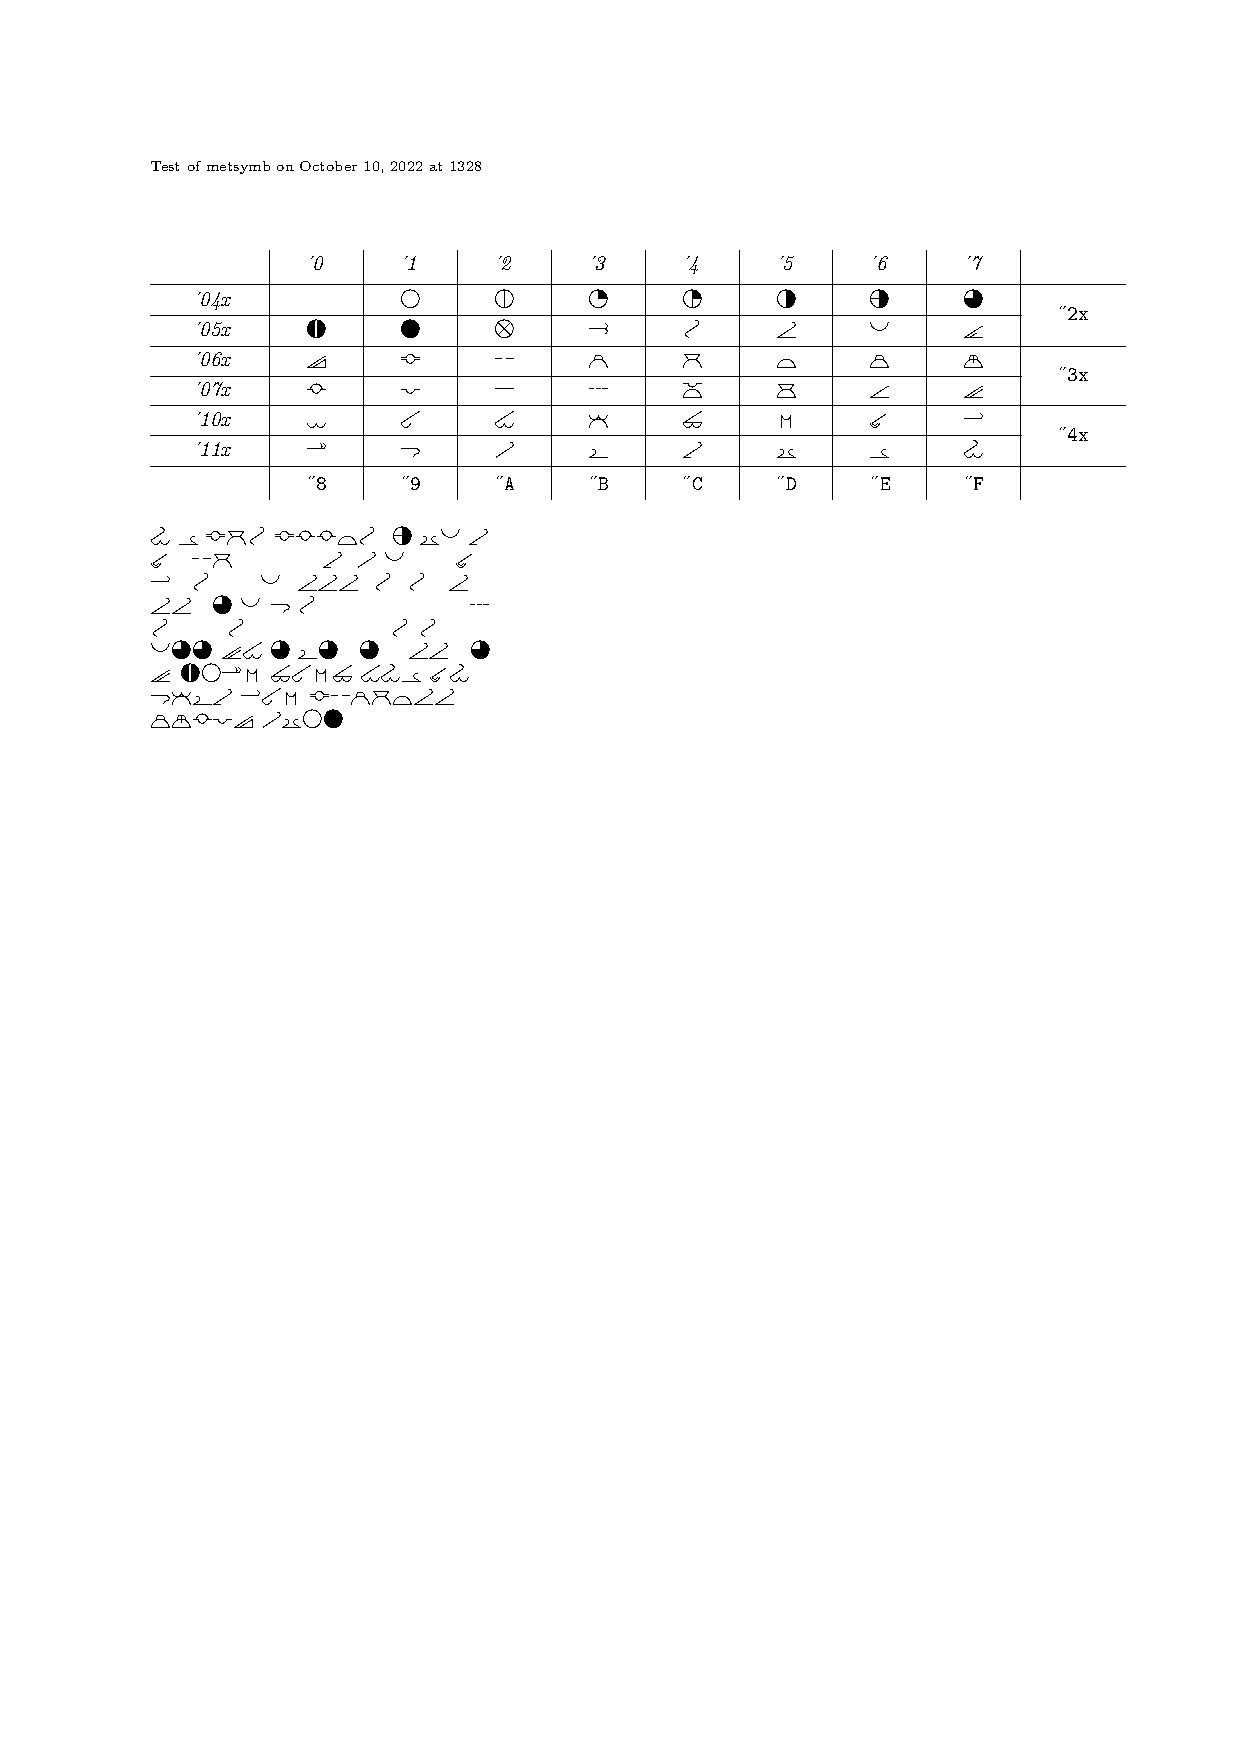
\includegraphics[scale=0.7]{testfont.pdf}}
% \caption{Complete font table for \textsf{metsymb}.}\label{fig:testfont}
% \end{figure}
%
% \StopEventually{\PrintIndex\PrintChanges}
%
% \section{Implementation}
%
% The \textsf{metsymb} package very simply defines new commands to fetch individual glyphs from the \texttt{metsymb} font. As such, its \LaTeX\ side is rather simple.
%
% \begin{macro}{\zerookta}
% The 0 okta symbol:
%    \begin{macrocode}
\newcommand{\zerookta}{{\usefont{U}{metsymb}{m}{n} \char33 }}%
%    \end{macrocode}
% \end{macro}
%
% \begin{macro}{\oneokta}
% The 1 okta symbol:
%    \begin{macrocode}
\newcommand{\oneokta}{{\usefont{U}{metsymb}{m}{n} \char34 }}%
%    \end{macrocode}
% \end{macro}
%
% \begin{macro}{\twooktas}
% The 2 oktas symbol:
%    \begin{macrocode}
\newcommand{\twooktas}{{\usefont{U}{metsymb}{m}{n} \char35 }}%
%    \end{macrocode}
% \end{macro}
%
% \begin{macro}{\threeoktas}
% The 3 oktas symbol:
%    \begin{macrocode}
\newcommand{\threeoktas}{{\usefont{U}{metsymb}{m}{n} \char36 }}%
%    \end{macrocode}
% \end{macro}
%
% \begin{macro}{\fouroktas}
% The 4 oktas symbol:
%    \begin{macrocode}
\newcommand{\fouroktas}{{\usefont{U}{metsymb}{m}{n} \char37 }}%
%    \end{macrocode}
% \end{macro}
%
% \begin{macro}{\fiveoktas}
% The 5 oktas symbol:
%    \begin{macrocode}
\newcommand{\fiveoktas}{{\usefont{U}{metsymb}{m}{n} \char38 }}%
%    \end{macrocode}
% \end{macro}
%
% \begin{macro}{\sixoktas}
% The 6 oktas symbol:
%    \begin{macrocode}
\newcommand{\sixoktas}{{\usefont{U}{metsymb}{m}{n} \char39 }}%
%    \end{macrocode}
% \end{macro}
%
% \begin{macro}{\sevenoktas}
% The 7 oktas symbol:
%    \begin{macrocode}
\newcommand{\sevenoktas}{{\usefont{U}{metsymb}{m}{n} \char40 }}%
%    \end{macrocode}
% \end{macro}
%
% \begin{macro}{\eightoktas}
% The 8 oktas symbol:
%    \begin{macrocode}
\newcommand{\eightoktas}{{\usefont{U}{metsymb}{m}{n} \char41 }}%
%    \end{macrocode}
% \end{macro}
%
% \begin{macro}{\nineoktas}
% The 9 oktas symbol:
%    \begin{macrocode}
\newcommand{\nineoktas}{{\usefont{U}{metsymb}{m}{n} \char42 }}%
%    \end{macrocode}
% \end{macro}
%
% \begin{macro}{\cirrus}
% The cirrus symbol:
%    \begin{macrocode}
\newcommand{\cirrus}{{\usefont{U}{metsymb}{m}{n} \char43 }}%
%    \end{macrocode}
% \end{macro}
%
% \begin{macro}{\cirrocumulus}
% The cirrocumulus symbol:
%    \begin{macrocode}
\newcommand{\cirrocumulus}{{\usefont{U}{metsymb}{m}{n} \char44 }}%
%    \end{macrocode}
% \end{macro}
%
% \begin{macro}{\cirrostratus}
% The cirrostratus symbol:
%    \begin{macrocode}
\newcommand{\cirrostratus}{{\usefont{U}{metsymb}{m}{n} \char45 }}%
%    \end{macrocode}
% \end{macro}
%
% \begin{macro}{\altocumulus}
% The altocumulus symbol:
%    \begin{macrocode}
\newcommand{\altocumulus}{{\usefont{U}{metsymb}{m}{n} \char46 }}%
%    \end{macrocode}
% \end{macro}
%
% \begin{macro}{\altostratus}
% The altostratus symbol:
%    \begin{macrocode}
\newcommand{\altostratus}{{\usefont{U}{metsymb}{m}{n} \char47 }}%
%    \end{macrocode}
% \end{macro}
%
% \begin{macro}{\nimbostratus}
% The nimbostratus symbol:
%    \begin{macrocode}
\newcommand{\nimbostratus}{{\usefont{U}{metsymb}{m}{n} \char48 }}%
%    \end{macrocode}
% \end{macro}
%
% \begin{macro}{\stratocumulus}
% The stratocumulus symbol:
%    \begin{macrocode}
\newcommand{\stratocumulus}{{\usefont{U}{metsymb}{m}{n} \char49 }}%
%    \end{macrocode}
% \end{macro}
%
% \begin{macro}{\stratus}
% The stratus symbol:
%    \begin{macrocode}
\newcommand{\stratus}{{\usefont{U}{metsymb}{m}{n} \char50 }}%
%    \end{macrocode}
% \end{macro}
%
% \begin{macro}{\cumulus}
% The cumulus symbol:
%    \begin{macrocode}
\newcommand{\cumulus}{{\usefont{U}{metsymb}{m}{n} \char51 }}%
%    \end{macrocode}
% \end{macro}
%
% \begin{macro}{\cumulonimbus}
% The cumulonimbus symbol:
%    \begin{macrocode}
\newcommand{\cumulonimbus}{{\usefont{U}{metsymb}{m}{n} \char52 }}%
%    \end{macrocode}
% \end{macro}
%
% \begin{macro}{\clI}
% The C$_\text{L}=1$ cloud symbol:
%    \begin{macrocode}
\newcommand{\clI}{{\usefont{U}{metsymb}{m}{n} \char53 }}%
%    \end{macrocode}
% \end{macro}
%
% \begin{macro}{\clII}
% The C$_\text{L}=2$ cloud symbol:
%    \begin{macrocode}
\newcommand{\clII}{{\usefont{U}{metsymb}{m}{n} \char54 }}%
%    \end{macrocode}
% \end{macro}
%
% \begin{macro}{\clIII}
% The C$_\text{L}=3$ cloud symbol:
%    \begin{macrocode}
\newcommand{\clIII}{{\usefont{U}{metsymb}{m}{n} \char55 }}%
%    \end{macrocode}
% \end{macro}
%
% \begin{macro}{\clIV}
% The C$_\text{L}=4$ cloud symbol:
%    \begin{macrocode}
\newcommand{\clIV}{{\usefont{U}{metsymb}{m}{n} \char56 }}%
%    \end{macrocode}
% \end{macro}
%
% \begin{macro}{\clV}
% The C$_\text{L}=5$ cloud symbol:
%    \begin{macrocode}
\newcommand{\clV}{{\usefont{U}{metsymb}{m}{n} \char57 }}%
%    \end{macrocode}
% \end{macro}
%
% \begin{macro}{\clVI}
% The C$_\text{L}=6$ cloud symbol:
%    \begin{macrocode}
\newcommand{\clVI}{{\usefont{U}{metsymb}{m}{n} \char58 }}%
%    \end{macrocode}
% \end{macro}
%
% \begin{macro}{\clVII}
% The C$_\text{L}=7$ cloud symbol:
%    \begin{macrocode}
\newcommand{\clVII}{{\usefont{U}{metsymb}{m}{n} \char59 }}%
%    \end{macrocode}
% \end{macro}
%
% \begin{macro}{\clVIII}
% The C$_\text{L}=8$ cloud symbol:
%    \begin{macrocode}
\newcommand{\clVIII}{{\usefont{U}{metsymb}{m}{n} \char60 }}%
%    \end{macrocode}
% \end{macro}
%
% \begin{macro}{\clIX}
% The C$_\text{L}=9$ cloud symbol:
%    \begin{macrocode}
\newcommand{\clIX}{{\usefont{U}{metsymb}{m}{n} \char61 }}%
%    \end{macrocode}
% \end{macro}
%
% \begin{macro}{\cmI}
% The C$_\text{M}=1$ cloud symbol:
%    \begin{macrocode}
\newcommand{\cmI}{{\usefont{U}{metsymb}{m}{n} \char62 }}%
%    \end{macrocode}
% \end{macro}
%
% \begin{macro}{\cmII}
% The C$_\text{M}=2$ cloud symbol:
%    \begin{macrocode}
\newcommand{\cmII}{{\usefont{U}{metsymb}{m}{n} \char63 }}%
%    \end{macrocode}
% \end{macro}
%
% \begin{macro}{\cmIII}
% The C$_\text{M}=3$ cloud symbol:
%    \begin{macrocode}
\newcommand{\cmIII}{{\usefont{U}{metsymb}{m}{n} \char64 }}%
%    \end{macrocode}
% \end{macro}
%
% \begin{macro}{\cmIV}
% The C$_\text{M}=4$ cloud symbol:
%    \begin{macrocode}
\newcommand{\cmIV}{{\usefont{U}{metsymb}{m}{n} \char65 }}%
%    \end{macrocode}
% \end{macro}
%
% \begin{macro}{\cmV}
% The C$_\text{M}=5$ cloud symbol:
%    \begin{macrocode}
\newcommand{\cmV}{{\usefont{U}{metsymb}{m}{n} \char66 }}%
%    \end{macrocode}
% \end{macro}
%
% \begin{macro}{\cmVI}
% The C$_\text{M}=6$ cloud symbol:
%    \begin{macrocode}
\newcommand{\cmVI}{{\usefont{U}{metsymb}{m}{n} \char67 }}%
%    \end{macrocode}
% \end{macro}
%
% \begin{macro}{\cmVII}
% The C$_\text{M}=7$ cloud symbol:
%    \begin{macrocode}
\newcommand{\cmVII}{{\usefont{U}{metsymb}{m}{n} \char68 }}%
%    \end{macrocode}
% \end{macro}
%
% \begin{macro}{\cmVIII}
% The C$_\text{M}=8$ cloud symbol:
%    \begin{macrocode}
\newcommand{\cmVIII}{{\usefont{U}{metsymb}{m}{n} \char69 }}%
%    \end{macrocode}
% \end{macro}
%
% \begin{macro}{\cmIX}
% The C$_\text{M}=9$ cloud symbol:
%    \begin{macrocode}
\newcommand{\cmIX}{{\usefont{U}{metsymb}{m}{n} \char70 }}%
%    \end{macrocode}
% \end{macro}
%
% \begin{macro}{\chI}
% The C$_\text{H}=1$ cloud symbol:
%    \begin{macrocode}
\newcommand{\chI}{{\usefont{U}{metsymb}{m}{n} \char71 }}%
%    \end{macrocode}
% \end{macro}
%
% \begin{macro}{\chII}
% The C$_\text{H}=2$ cloud symbol:
%    \begin{macrocode}
\newcommand{\chII}{{\usefont{U}{metsymb}{m}{n} \char72 }}%
%    \end{macrocode}
% \end{macro}
%
% \begin{macro}{\chIII}
% The C$_\text{H}=3$ cloud symbol:
%    \begin{macrocode}
\newcommand{\chIII}{{\usefont{U}{metsymb}{m}{n} \char73 }}%
%    \end{macrocode}
% \end{macro}
%
% \begin{macro}{\chIV}
% The C$_\text{H}=4$ cloud symbol:
%    \begin{macrocode}
\newcommand{\chIV}{{\usefont{U}{metsymb}{m}{n} \char74 }}%
%    \end{macrocode}
% \end{macro}
%
% \begin{macro}{\chV}
% The C$_\text{H}=5$ cloud symbol:
%    \begin{macrocode}
\newcommand{\chV}{{\usefont{U}{metsymb}{m}{n} \char75 }}%
%    \end{macrocode}
% \end{macro}
%
% \begin{macro}{\chVI}
% The C$_\text{H}=6$ cloud symbol:
%    \begin{macrocode}
\newcommand{\chVI}{{\usefont{U}{metsymb}{m}{n} \char76 }}%
%    \end{macrocode}
% \end{macro}
%
% \begin{macro}{\chVII}
% The C$_\text{H}=7$ cloud symbol:
%    \begin{macrocode}
\newcommand{\chVII}{{\usefont{U}{metsymb}{m}{n} \char77 }}%
%    \end{macrocode}
% \end{macro}
%
% \begin{macro}{\chVIII}
% The C$_\text{H}=8$ cloud symbol:
%    \begin{macrocode}
\newcommand{\chVIII}{{\usefont{U}{metsymb}{m}{n} \char78 }}%
%    \end{macrocode}
% \end{macro}
%
% \begin{macro}{\chIX}
% The C$_\text{H}=9$ cloud symbol:
%    \begin{macrocode}
\newcommand{\chIX}{{\usefont{U}{metsymb}{m}{n} \char79 }}%
%    \end{macrocode}
% \end{macro}
%
% \Finale
\endinput